\section{Ilustrações, tabelas e outros objetos acadêmicos}\label{sec:catalogo-exemplos}

Esta seção funciona como catálogo visual e corpus de regressão. Cada grupo apresenta primeiro a regra ou política exercitada e, em seguida, exemplos compiláveis. Os objetos devem ser citados e discutidos no texto do trabalho real; não devem ser incluídos apenas para preencher o documento.

\subsection{Regra geral para ilustrações}

\guianormativa{ABNT NBR 14724:2024 e NBR 10520:2023}{Ilustrações devem ser identificadas de modo consistente e apresentar indicação de fonte. Quando a fonte for externa, sua indicação deve ser compatível com o sistema de citações adotado \parencite{abnt14724,abnt10520}.}

\guiapolitica{Na V2, título, fonte e nota são vinculados à largura física do objeto. Os testes verificam que esses elementos não ultrapassem horizontalmente a largura da ilustração. O tamanho reduzido adotado para títulos e fontes de objetos é 10 pt no escopo institucional do projeto.}

\subsection{Figuras em diferentes larguras e formatos}

\legend{figure}{Figura estreita com legenda curta}
\ufcfonte{Elaboração própria.}
\label{fig:estreita}
\begin{ufcobjeto}[here]
  \centering
  \fbox{\parbox[c][2.6cm][c]{5.5cm}{\centering Figura sintética\\5,5 cm}}
\end{ufcobjeto}

\guiaexemplo{A Figura~\ref{fig:estreita} demonstra que uma figura estreita não deve fazer seu título ou sua fonte ocuparem arbitrariamente toda a mancha gráfica.}

\legend{figure}{Figura de largura intermediária com uma legenda deliberadamente longa para validar quebra de linha, alinhamento e limite horizontal do título do objeto}
\ufcfonte{Elaboração própria.}
\ufcnota{Exemplo sintético usado para verificar título, fonte e nota em um objeto de largura intermediária.}
\label{fig:media}
\begin{ufcobjeto}[here]
  \centering
  \fbox{\parbox[c][3cm][c]{9cm}{\centering Figura sintética de largura intermediária\\9 cm}}
\end{ufcobjeto}

\legend{figure}{Figura larga próxima à largura útil da mancha gráfica}
\ufcfonte{Elaboração própria.}
\label{fig:larga}
\begin{ufcobjeto}[here]
  \centering
  \fbox{\parbox[c][3cm][c]{0.78\linewidth}{\centering Figura sintética larga\\78\% da largura disponível}}
\end{ufcobjeto}

\legend{figure}{Fluxo de processamento em arquivo PNG raster}
\ufcfonte{Elaboração própria.}
\ufcnota{O arquivo é incluído diretamente com \texttt{\string\includegraphics}.}
\label{fig:png-fluxo}
\begin{ufcobjeto}[here]
  \centering
  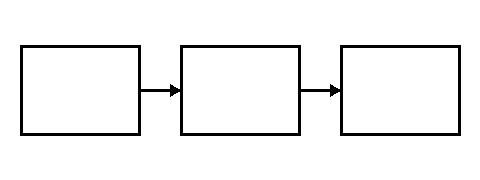
\includegraphics[width=0.65\linewidth]{figures/example-flow.png}
\end{ufcobjeto}

As Figuras~\ref{fig:media}, \ref{fig:larga} e~\ref{fig:png-fluxo} exercitam larguras progressivamente maiores, quebra de título, fonte, nota e inclusão de imagem raster.

\subsection{Imagens institucionais reais da UFC}

\legend{figure}{Campus do Pici, onde se localiza o Departamento de Computação da UFC}
\ufcfonte{Universidadefederalceara (2018), Wikimedia Commons, CC BY-SA 4.0.}
\ufcnota{Vista da Lagoa do Pici no Campus do Pici.}
\label{fig:campus-pici-computacao}
\begin{ufcobjeto}[here]
  \centering
  \IfFileExists{figures/ufc-campus-pici.jpg}
    {\includegraphics[width=0.72\linewidth]{figures/ufc-campus-pici.jpg}}
    {\fbox{\parbox[c][4cm][c]{0.72\linewidth}{\centering Execute \texttt{make reference-assets} para baixar a fotografia licenciada do Campus do Pici.}}}
\end{ufcobjeto}

\legend{figure}{Reitoria da Universidade Federal do Ceará}
\ufcfonte{Joelkaula (2018), Wikimedia Commons, CC BY-SA 4.0.}
\ufcnota{Fotografia externa usada sem modificação e distribuída sob licença própria; ver \texttt{figures/LICENSES.md}.}
\label{fig:reitoria-ufc}
\begin{ufcobjeto}[here]
  \centering
  \IfFileExists{figures/ufc-reitoria.jpg}
    {\includegraphics[width=0.62\linewidth]{figures/ufc-reitoria.jpg}}
    {\fbox{\parbox[c][5cm][c]{0.62\linewidth}{\centering Execute \texttt{make reference-assets} para baixar a fotografia licenciada da Reitoria da UFC.}}}
\end{ufcobjeto}

\guiapolitica{Fotografias externas de demonstração não são incorporadas aos bundles públicos/CTAN sem controle de licença. O comando \texttt{make reference-assets} baixa os arquivos de referência e verifica sua integridade; as licenças ficam registradas separadamente.}

\subsection{Gráficos}

Gráficos são tratados como ilustrações e participam da Lista de Ilustrações no modelo de referência.

\legend{grafico}{Distribuição sintética de três categorias}
\ufcfonte{Elaboração própria.}
\ufcnota{Valores meramente ilustrativos.}
\label{graf:barras}
\begin{ufcobjeto}[here]
  \centering
  \begingroup
  \setlength{\unitlength}{1pt}
  \begin{picture}(300,180)
    \put(45,25){\line(1,0){235}}
    \put(45,25){\line(0,1){130}}
    \put(40,25){\makebox(0,0)[r]{0}}
    \put(40,58){\makebox(0,0)[r]{5}}
    \put(40,90){\makebox(0,0)[r]{10}}
    \put(40,123){\makebox(0,0)[r]{15}}
    \put(40,155){\makebox(0,0)[r]{20}}
    \put(45,58){\line(1,0){235}}
    \put(45,90){\line(1,0){235}}
    \put(45,123){\line(1,0){235}}
    \put(45,155){\line(1,0){235}}
    \put(76,25){\color{black!55}\rule{35pt}{78pt}}
    \put(148,25){\color{black!55}\rule{35pt}{117pt}}
    \put(220,25){\color{black!55}\rule{35pt}{59pt}}
    \put(94,109){\makebox(0,0){12}}
    \put(166,148){\makebox(0,0){18}}
    \put(238,90){\makebox(0,0){9}}
    \put(94,12){\makebox(0,0){Categoria A}}
    \put(166,12){\makebox(0,0){Categoria B}}
    \put(238,12){\makebox(0,0){Categoria C}}
    \put(165,0){\makebox(0,0){Categoria}}
    \put(8,90){\rotatebox{90}{Valor}}
  \end{picture}
  \endgroup
\end{ufcobjeto}

\guiaexemplo{O Gráfico~\ref{graf:barras} é desenhado diretamente em \LaTeX{} para que a regressão visual não dependa de um arquivo externo. Em uma pesquisa real, escolha o tipo de gráfico de acordo com os dados e informe claramente escalas, unidades, categorias e fonte.}

\subsection{Quadros}

O projeto distingue quadros de tabelas numéricas. Quadros são úteis para organizar conteúdo predominantemente textual.

\legend{quadro}{Comparação de configurações editoriais do exemplo}
\ufcfonte{Elaboração própria.}
\label{qua:configuracoes}
\begin{ufcobjeto}[here]
  \centering
  \begin{tabular}{lll}
    \hline
    Elemento & Variação A & Variação B \\
    \hline
    Figura & estreita & larga \\
    Código & sem linhas & com linhas \\
    Algoritmo & sem linhas & com linhas \\
    \hline
  \end{tabular}
\end{ufcobjeto}

\guiaexemplo{O Quadro~\ref{qua:configuracoes} demonstra informação textual organizada em linhas e colunas. Não use a denominação ``tabela'' apenas porque um conteúdo foi produzido com o ambiente \texttt{tabular}; a escolha do tipo deve considerar a natureza da informação apresentada.}

\subsection{Tabelas numéricas}

\guianormativa{Normas de Apresentação Tabular do IBGE, 3. ed.}{Para tabelas numéricas, a V2 exercita laterais abertas, ausência de grade no corpo e regras horizontais superior, de separação do cabeçalho e inferior \parencite{ibge1993}.}

\begin{table}[htbp]
\centering
\begin{tallabnttblr}
[
  caption={Indicadores sintéticos com linhas alternadas},
  label={tab:zebra},
  remark{Fonte}={Elaboração própria.},
  remark{Nota}={A alternância de fundo é opcional e usada aqui apenas como exemplo editorial.},
]
{
  colspec={X[l] X[c] X[r]},
  row{even}={bg=black!5},
}
\toprule
Indicador & Ano & Valor \\
\midrule
Alfa & 2024 & 10 \\
Beta & 2025 & 12 \\
Gama & 2026 & 15 \\
Delta & 2026 & 18 \\
\bottomrule
\end{tallabnttblr}
\end{table}

\guiapolitica{A alternância de fundo da Tabela~\ref{tab:zebra} é uma extensão editorial opcional. Ela não é tratada como regra automática da ABNT ou do IBGE. O exemplo existe para mostrar que o módulo pode aplicar estilos sem alterar as regras estruturais da tabela.}

\subsection{Código-fonte}

Código-fonte não é convertido artificialmente em uma regra ABNT específica. A V2 o trata como objeto acadêmico com identificação, fonte, numeração e largura controladas, oferecendo módulos de apresentação configuráveis.

\guiapolitica{O documento de referência usa \texttt{listings}. A política de numeração das linhas pode variar conforme a finalidade do exemplo; o importante é manter legibilidade, identificação consistente e fonte do conteúdo quando aplicável.}

\lstset{language=Python,numbers=left,stepnumber=1,numbersep=8pt}
\legend{codigo}{Função de média em Python com números de linha}
\ufcfonte{Elaboração própria.}
\label{cod:python-numerado}
\begin{ufclisting}[here]
def media(valores):
    return sum(valores) / len(valores)
\end{ufclisting}

\lstset{language=C++,numbers=none}
\legend{codigo}{Função de máximo em C++ sem números de linha}
\ufcfonte{Elaboração própria.}
\label{cod:cpp-sem-numero}
\begin{ufclisting}[here]
int maximo(int a, int b) {
    return a > b ? a : b;
}
\end{ufclisting}

\legend{codigo}{Arquivo Python externo com números de linha}
\ufcfonte{Elaboração própria.}
\label{cod:python-externo}
\begin{ufcobjeto}[here]
  \ufcinputlisting[language=Python,numbers=left,numbersep=8pt]{figures/example.py}
\end{ufcobjeto}

\lstset{language=Java,numbers=left,stepnumber=2,numbersep=8pt}
\legend{codigo}{Método Java com numeração a cada duas linhas}
\ufcfonte{Elaboração própria.}
\label{cod:java}
\begin{ufclisting}[here]
static int dobro(int valor) {
    int resultado = 2 * valor;
    return resultado;
}
\end{ufclisting}
\lstset{numbers=none,stepnumber=1}

Os Códigos~\ref{cod:python-numerado}, \ref{cod:cpp-sem-numero}, \ref{cod:python-externo} e~\ref{cod:java} demonstram linguagens e políticas de numeração distintas usando o mesmo módulo.

\subsection{Algoritmos}

Algoritmos em pseudocódigo são apresentados como objetos próprios da V2. O módulo recomendado no documento de referência é \texttt{algpseudocodex}.

\guiapolitica{Numeração de linhas em pseudocódigo é uma opção editorial do exemplo e não uma exigência normativa geral. A identificação e a fonte continuam sendo tratadas de forma consistente com os demais objetos do template.}

\legend{algoritmo}{Máximo divisor comum com números de linha}
\ufcfonte{Elaboração própria.}
\label{alg:mdc-numerado}
\begin{ufcalgoritmo}[here][1]
  \While{$b \neq 0$}
    \State $r \gets a \bmod b$
    \State $a \gets b$
    \State $b \gets r$
  \EndWhile
  \State \Return $a$
\end{ufcalgoritmo}

\legend{algoritmo}{Seleção do maior valor sem números de linha}
\ufcfonte{Elaboração própria.}
\label{alg:maior-sem-numero}
\begin{ufcalgoritmo}[here][0]
  \If{$a > b$}
    \State \Return $a$
  \Else
    \State \Return $b$
  \EndIf
\end{ufcalgoritmo}

\subsection{Equações}

A Equação~\ref{eq:media-exemplo} exemplifica uma expressão numerada e referenciada no texto.
\begin{equation}
  \bar{x} = \frac{1}{n}\sum_{i=1}^{n}x_i
  \label{eq:media-exemplo}
\end{equation}

\guiapolitica{Use numeração e referência quando a equação precisar ser identificada no texto. A suíte matemática verifica a estabilidade tipográfica e a integração do conteúdo matemático com os motores suportados.}

\subsection{Citação longa, alíneas e enumerações}

Uma citação direta longa também é exercitada no documento de referência. O conteúdo abaixo é sintético e existe apenas para permitir a verificação geométrica do bloco:

\Enquote{A composição tipográfica de um documento científico deve ser tratada como parte de um processo reprodutível de edição, revisão e validação, mantendo conteúdo e apresentação suficientemente separados para que mudanças editoriais possam ser verificadas de forma sistemática.}
\guianormativa{ABNT NBR 10520:2023}{O bloco acima exercita a apresentação de citação direta longa descrita na Seção~\ref{sec:citacoes-referencias}: recuo de 4 cm, fonte reduzida, espaço simples e ausência de aspas no PDF final \parencite{abnt10520}.}

Exemplo de alíneas e subalíneas:

\begin{ufcalineas}
  \item primeiro item de validação;
  \item segundo item de validação:
    \begin{ufcsubalineas}
      \item subitem de validação.
    \end{ufcsubalineas}
\end{ufcalineas}

Exemplo de enumeração comum:

\begin{enumerate}
  \item preparar o conteúdo;
  \item compilar o documento;
  \item revisar o PDF produzido.
\end{enumerate}

\subsection{Tipos bibliográficos exercitados}

O arquivo \texttt{backmatter/references.bib} reúne livro, artigo, evento, dissertação, relatório, normas e recursos eletrônicos. Campos como \texttt{isbn}, \texttt{doi}, \texttt{url}, \texttt{urldate}, \texttt{institution}, \texttt{edition}, \texttt{volume}, \texttt{number} e \texttt{pages} são usados apenas quando pertinentes ao tipo de documento.

\nocite{lamport1994,wessberg2000,vaswani2017attention,almeida2018,rfc9110}

\index{figuras}\index{gráficos}\index{quadros}\index{tabelas}\index{código-fonte}\index{algoritmos}\index{equações}
